\documentclass[19pt,landscaoe]{article}
\usepackage[landscape]{geometry}
\geometry{a5paper,scale=0.8}
%\geometry{left=1.5cm,right=1.5cm,top=1.5cm,bottom=0.5cm}
\usepackage{color}
% \usepackage{ulem} % for strikethrough
\usepackage{amsfonts}
\usepackage{bm}
\usepackage{Sweave}
\usepackage{graphicx} 
\usepackage{amsfonts,amsmath,latexsym,amssymb,mathrsfs,amsthm,mathtools}
% \usepackage[british]{babel}
%\usepackage[T1]{fontenc}
%\usepackage{mathptmx}
% \usepackage{times}
\usepackage{datetime2}
\usepackage{filemod}
% \usepackage{fontspec}    %change font 
% \setmainfont{Times New Roman}%fontspec下这个命令设置全局默认字体
\newtheorem{thm}{Theorem}%[section]
\newtheorem{prop}[thm]{Proposition}
\newtheorem{defi}[thm]{Definition}
\newtheorem{lma}[thm]{Lemma}
\newtheorem{cor}[thm]{Corollary}
\newtheorem{exam}[thm]{Example}
\newtheorem{countexam}[thm]{Counterexample}
\newtheorem{rem}[thm]{Remark}
\newtheorem{con}[thm]{Conjecture}
%\bracketfactory{floor}{\lfloor}{\rfloor}
\usepackage{enumerate}
\usepackage{color}
%\usetheme{Copenhagen}
\usepackage[english]{babel}
\usepackage[utf8x]{inputenc}
\newcommand{\law}{\mathscr{L}}
\newcommand{\HH}{\mathscr{H}}
\newcommand{\D}{\mathbb{D}}
\newcommand{\IP}{\mathbb{P}} 
\newcommand{\bone}{{\bf 1}}
\DeclareMathOperator{\E}{\mathbb{E}}
\DeclareMathOperator*{\esssup}{ess\,sup}
\newcommand{\IE}{\E}
\newcommand{\mean}{\E}
\newcommand{\R}{\mathbb{R}}
\newcommand{\N}{\mathbb{N}}
\newcommand{\non}{\nonumber}
\newcommand{\Z}{\mathbb{Z}}
\newcommand{\C}{\mathbb{C}}
%\newcommand{\C}{{\mathds{C}}}
\newcommand{\ci}{{\cal I}}
\newcommand{\cf}{{\cal F}}
\newcommand{\LL}{\textbf{L}}
\DeclareMathOperator{\Var}{\mathrm{Var}}
\DeclareMathOperator{\var}{\mathrm{Var}}
\DeclareMathOperator{\cov}{\mathrm{Cov}}
\DeclareMathOperator{\corr}{\mathrm{Corr}}
\DeclareMathOperator{\bigo}{\mathrm{O}}
\newcommand{\K}{\textbf{Ker}}
\newcommand{\Id}{\textbf{Id}}
\newcommand{\Pn}{{\rm Pn}}
\newcommand{\dtv}{{d_{\rm TV}}}
\newcommand{\dk}{{d_{\rm K}}}
\newcommand{\dw}{{d_{\rm W}}}
\def\tg{{\tilde g}}
\def\a{{\alpha}}
\def\cn{{\mathcal{N}}}
\def\equald{\stackrel{\mbox{\scriptsize{{\rm d}}}}{=}}
\def\ER{Erd\H{o}s-R\'enyi}
\usepackage{color} 
\definecolor{lightblue}{rgb}{0,0.2,0.5}
\usepackage[colorlinks=true, urlcolor=lightblue,linkcolor=lightblue, citecolor=lightblue]{hyperref}

%%%%%%%%%%%%%%%%%%%%%%%%%%%%%%%%%%

%%% Define bracket commands
\def\given{\mskip 0.5mu plus 0.25mu\vert\mskip 0.5mu plus 0.15mu}
\newcounter{@bracketlevel}
\def\@bracketfactory#1#2#3#4#5#6{
\expandafter\def\csname#1\endcsname##1{%
\addtocounter{@bracketlevel}{1}%
\global\expandafter\let\csname @middummy\alph{@bracketlevel}\endcsname\given%
\global\def\given{\mskip#5\csname#4\endcsname\vert\mskip#6}\csname#4l\endcsname#2##1\csname#4r\endcsname#3%
\global\expandafter\let\expandafter\given\csname @middummy\alph{@bracketlevel}\endcsname
\addtocounter{@bracketlevel}{-1}}%
}
\def\bracketfactory#1#2#3{%
\@bracketfactory{#1}{#2}{#3}{relax}{0.5mu plus 0.25mu}{0.5mu plus 0.15mu}
\@bracketfactory{b#1}{#2}{#3}{big}{1mu plus 0.25mu minus 0.25mu}{0.6mu plus 0.15mu minus 0.15mu}
\@bracketfactory{bb#1}{#2}{#3}{Big}{2.4mu plus 0.8mu minus 0.8mu}{1.8mu plus 0.6mu minus 0.6mu}
\@bracketfactory{bbb#1}{#2}{#3}{bigg}{3.2mu plus 1mu minus 1mu}{2.4mu plus 0.75mu minus 0.75mu}
\@bracketfactory{bbbb#1}{#2}{#3}{Bigg}{4mu plus 1mu minus 1mu}{3mu plus 0.75mu minus 0.75mu}
}


% \title{Nonparametric Regression}
% \author{Qingwei Liu}
% \institute{National University of Singapore}
% \date{\today}

\begin{document}
% \maketitle
%

\begin{titlepage}
\begin{center}
    \vfill
\textbf{\huge ST5207 Nonparametric Regression\\
Semester 1, AY2024/25}\\[4cm]
\begin{minipage}{0.4\textwidth}
\begin{center} \large
Lecturer:~Qingwei Liu\\
% Email:liu\_qw@nus.edu.sg\\
\vskip 6pt
Department of Statistics and Data Science\\
\vskip 6pt
National University of Singapore
\end{center}
\end{minipage}%\\[1cm]
\vfill
% \includegraphics[width=0.1\textwidth]{./logo}\\[0.5cm]
\vfill
\end{center}

\end{titlepage}
%
\newpage
{\LARGE\centerline{\textbf {Administration}\footnote{Last modified in \filemodprintdate{Lecture1}.}}}
\vskip25pt
\begin{minipage}{.9\textwidth}
    \Large
\begin{itemize}
\item Course website: Accessible through \href{https://www.nus.edu.sg/canvas/login/}{Canvas} for lecture slides, assignments, solutions, etc. 
\item Prerequisites: Probability and Mathematical Statistics 
\item Consultation: via \href{mailto:liu_qw@nus.edu.sg}{ email} \& appointment via email
\item a 2-hour lecture + 1-hour tutorial per week
\item Homework
\item Assessment: Final exam ($60\%$) + Assignments ($40\%$)
\item Main reference are \cite{hardle04} \& \cite{scott15}. 
\item Reference include \cite{simonoff12}, \cite{takezawa05}, \cite{wasserman}, \cite{Hall13}, and \cite{kloke14}.

\end{itemize}
\end{minipage}
\newpage
{\LARGE\centerline{\textbf{Lecture~1:~Introduction}}}
\vskip25pt
\begin{minipage}{.9\textwidth}
    \Large
    The course is about various {\it smoothing} methods for estimating the probability density functions (p.d.f.) and the conditional mean functions (or regression)
\begin{enumerate}[(i)]
\item Get an overview of nonparametric methods
\begin{enumerate}[a)]
    \item Empirical distribution function;
    \item density estimation
    \item Nadaraya-Watson kernel regression;
    \item and other methods...
\end{enumerate}
\item Understand the pros and cons of each methods
\item Understand basic theories behind nonparametric methods
\item R packages
\end{enumerate}
\end{minipage}
\newpage
{\Large\centerline{\textbf{Parametric v.s. Nonparametric}}}
\vskip25pt
\begin{minipage}{.9\textwidth}
    \Large
Two distinct approaches of modelling and inference. 
\vskip 5pt
Let $X_1,\dots,X_n$ be a sequence of independent and identical distributed (i.i.d.) random variables with a common cumulative distribution function (c.d.f.) $F$. Alternatively, we write $X_1,\dots,X_n\overset{\mathrm{i.i.d.}}{\sim}F$. \\Assume the distribution function $F$ has a density function $$f(x)=\frac{\mathrm{d}F(x)}{\mathrm{d}x}.$$  
The parametric approach for density estimation assmues known function forms of $F$ or $f$ which involves some unknown {\bf parameters}.\\ We may write
$$F(x)=F_\theta(x)=F(x|\theta).$$
One has to make prior assumptions about its functional form.
\end{minipage}
\newpage
{\LARGE\centerline{\textbf{Nonparametric approach }}}
\vskip25pt
\begin{minipage}{.9\textwidth}
    \Large

Nonparametric inference requires weaker assumptions, for instance, 
\vfill
\begin{itemize}
\item $X_1,\dots,X_n$ are i.i.d. and $\E(X_1^2)<\infty$;
\item Or $X_1,\dots,X_n$ are i.i.d. with the $r$-th derivative $f^{(r)}(x)$ of the density exists, for certain $r>0$;
\item No assumptions about specific forms of the density $f$.
\end{itemize}
More specifically, {\bf given} a parametric density family $f(x|\theta)$, e.g. normal distribution $\mathcal{N}(\mu,\sigma^2)$ with unknown parameter $\theta=(\mu,\sigma^2)$, the emphasis in the parametric estimation is on obtaining the best estimator $\hat{\theta}$ of $\theta$. While the emphasis in nonparametric approach is directly on obtaining a good estimation $\hat{f}(\cdot)$ of the {\it entire} density function $f$.
\end{minipage}

\newpage
{\LARGE\centerline{\textbf{Mathematical formulation of regressions}}}
\vskip25pt
\Large
\begin{minipage}{.9\textwidth}
    \begin{enumerate}[(A)]
        \item response: $Y$; predictors (regressors, covariate): $X = (\mathbf{x}_1, ..., \mathbf{x}_p) $
        \item The interest is to find
        $
         E(Y|X=x)
        $
        i.e. the mean of $ Y$ when $ X =x$.
        \item Question: how to estimate $E(Y|X=x)$ if you can get whatever data $(X, Y)$?
        \begin{enumerate}[(a)]
        \item if you can repeatedly observe $ Y$ with $ X = x$?
        \item if you CANNOT repeatedly observe $ Y$ with $ X = x$ (which is more practical)?  --- this is the interest of statistics, data science, and computer sciences,... it is also our interest of this module
        
        
        \end{enumerate}
        
        \end{enumerate}
        
\end{minipage}

\newpage
{\LARGE\centerline{\textbf{``Local'' and ``Global'' Approaches to the estimation}}}
\vskip25pt
\large
% \begin{minipage}{.9\textwidth}
    \begin{enumerate}[(A)]

        \item Suppose we have observations $(X_i, y_i), i = 1, ..., n $
        
        \item ``Local'': if $ X=x $ is not repeatedly  observed, we can use those observations around $ x $: for example $ ||x_i - x|| \le h $, where $ h $ is small value and estimate
            $$
             \widehat{{E(Y|X=x)}} = \frac{1}{\#\{x_i: ||X_i - x|| \le h\}} \sum_{x_i: ||X_i - x|| \le h} Y_i
            $$
            where $ \#A $ denotes the number of elements in set A.\\

            {\bf Example 1:} Motorcycle data, the crashed effects after the motorcycles hit by a stimulated impact.  X: time after a stimulated impact with motorcycles; Y: head acceleration of a PTMO (post mortem human test object), capturing the crash effects.
            \begin{Schunk}
            \begin{Sinput}
library(MASS)
y=mcycle$accel
x=mcycle$times
plot(x,y, col = "red", main = "Motocycle Data", sub = 
"crashed effects after a stimulated impact", xlab = "Time",
 ylab = "acceleration")
            \end{Sinput}
        \end{Schunk}
        \begin{center}
            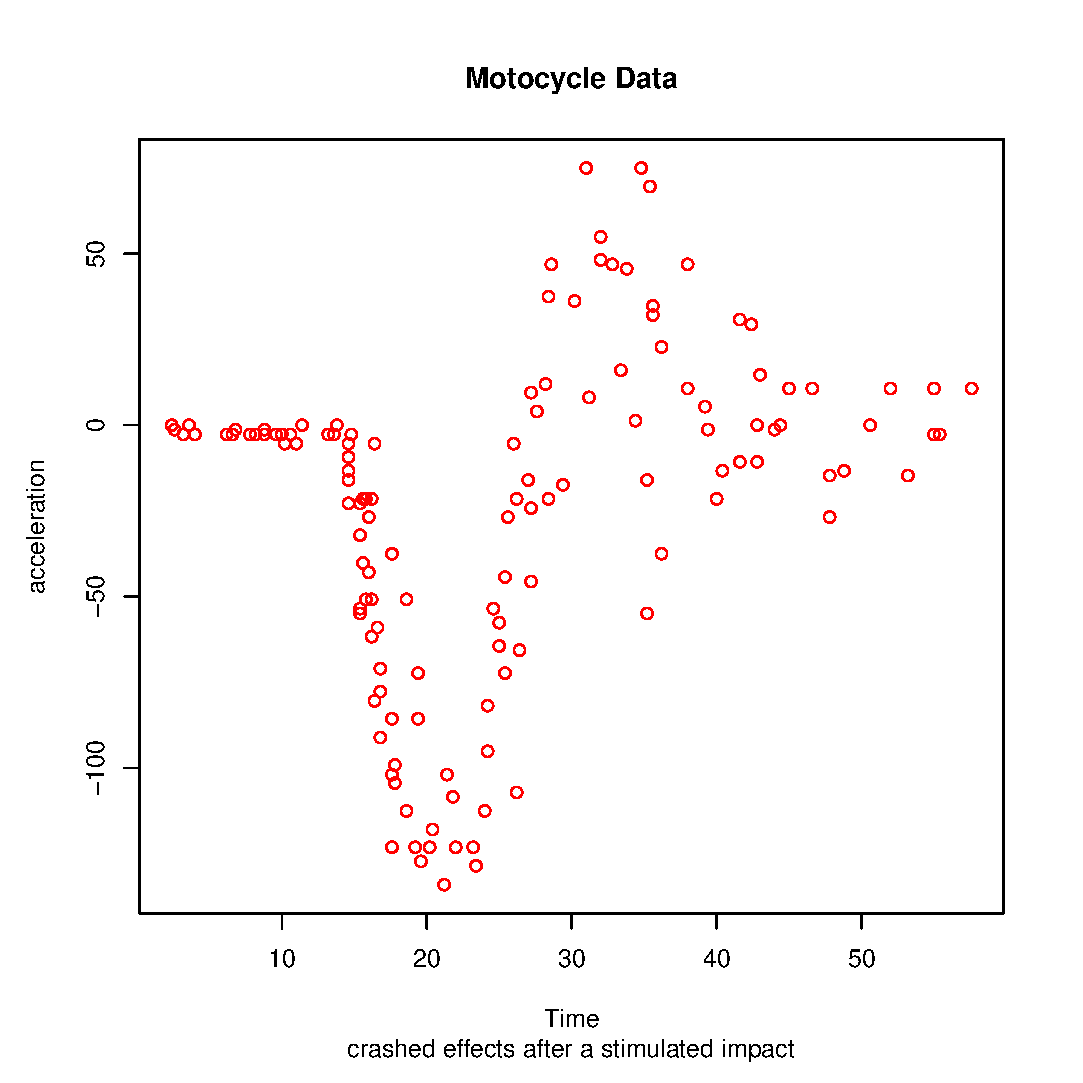
\includegraphics[width=0.6\textwidth,height=0.5\textwidth]{MotocycleData.eps}
        \end{center}
            \item ``local" approach to multivariate regressors, when $p $ increases, the number of observations in the neighbor  $ ||x_i - x|| \le h $ decreases dramatically. This leads to the ``curse of dimensionality".
            \item ``local" methods include
            \begin{enumerate}[(a)]
            
            \item ``k-nearest neighbors" or kNN
            
            \item Nadaraya-Watson kernel smoothing and its extensions
            
            \item regression tree and Random Forest
            
            \end{enumerate}
            \item ``global" approach assume
$$
E(Y|X=x)  = g(x, \beta)
$$
where $\beta$ is a set of parameters.

\item Examples:

\begin{enumerate}[(a)]

\item polynomial regression model: $ E(Y|X=x) = \beta_0 + \beta_1 x  + ... + \beta_m x^m $;
\begin{center}
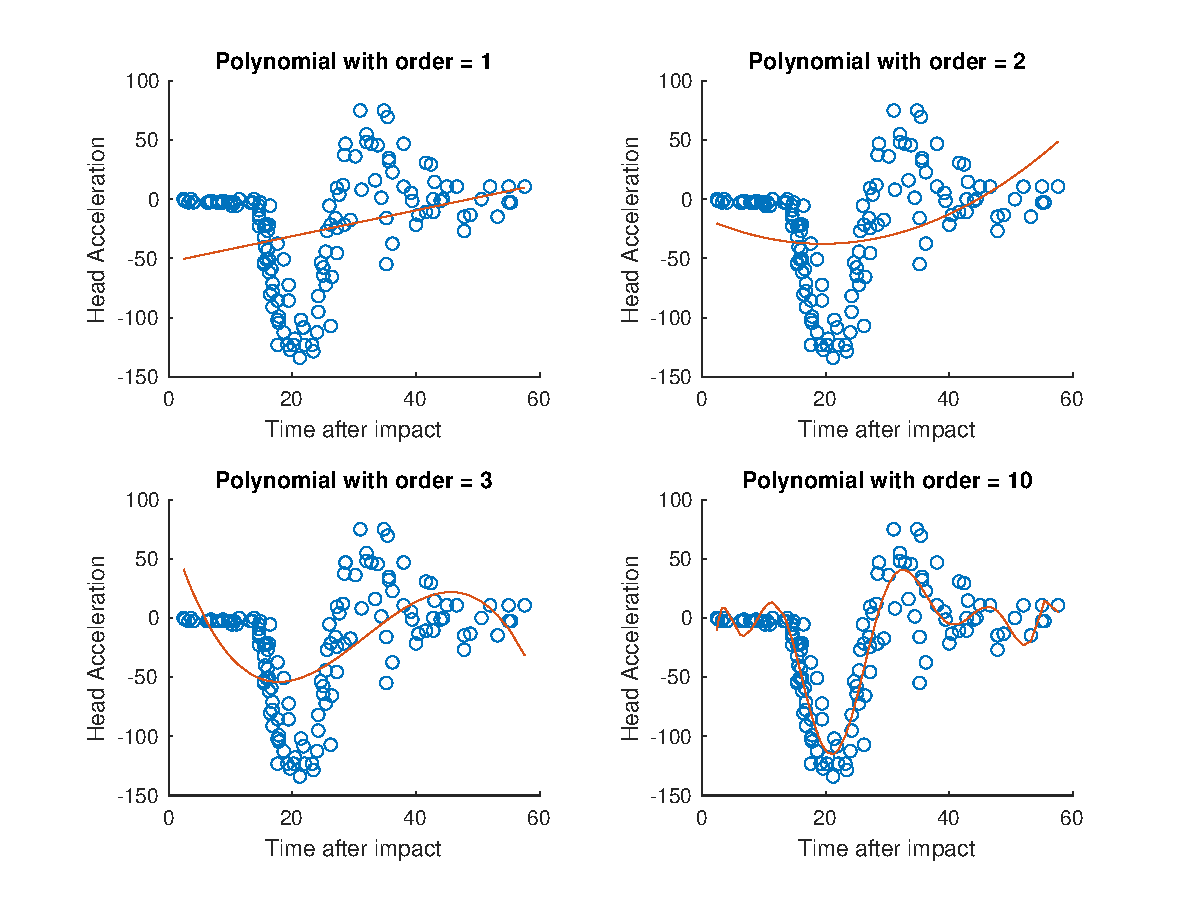
\includegraphics[width=0.6\textwidth,height=0.35\textwidth]{polyfitting.eps}
\end{center}
\item logistic regression model
$$
  E(y|x) = \frac{\exp(\beta_0 + \beta_1 x)}{1+\exp(\beta_0 + \beta_1 x)}
$$
Can you make this model more complicated?

\textbf{Example}
$$
  E(y|x) = c_1 \frac{\exp(\beta^{1}_0 + \beta^{1}_1 x)}{1+\exp(\beta^{1}_0 + \beta^{1}_1 x)} + c_2 \frac{\exp(\beta^{2}_0 + \beta^{2}_1 x)}{1+\exp(\beta^{2}_0 + \beta^{2}_1 x)}
$$
 or more complicated?  ---leading to the ANN
\item piece-wise linear: here we only consider univariate $ x $:
$$ E(Y|X=x) = \beta_0 + \beta_1 (x-t_1)_+ + \beta_2 (x-t_2)_+  + ... + \beta_m (x-t_m)_+ $$
Can you make this model more complicated?
\begin{enumerate}[(i)]
    \item Example 1:
    $$ E(Y|X=x) = \beta_0 + \alpha_1 x + \alpha_2 x^2 + \beta_1 (x-t_1)^3_+ + \beta_2 (x-t_2)^3_+  + ... + \beta_m (x-t_m)^3_+ $$
    or more complicated?  ---leading to the spline smoothing
    
    \item Example 2:
    $$ E(Y|X=x) = \beta_0 + \alpha_1 \phi_1(x) + \beta_1 \phi_2(x) + ....  $$
    where $ \phi_k(x), k = 1, 2, ... $ are a series of functions  ---leading to the Orthogonal Series Methods, including the wavelet, ...    
    \end{enumerate}

\end{enumerate}
\item Roughly speaking\footnote{not a formal defition}, if the number of parameters is fixed, we call the model parametric model, if the number increases with $n$, we call it  nonparametric model

\item "global" approaches to nonparametric regressions
\begin{enumerate}[(a)]

\item regression splines

\centerline{\includegraphics[width=8cm]{splinefit.pdf}}

\newpage 
\item orthogonal series methods

\item Reproducing kernel Hilbert space (RKHS) method

\item Artificial neural network (ANN) and deep-learning

\end{enumerate}

\item for ``global" approaches to multivariate regression, the curse of dimensionality still exists, but some methods have the adaptivity to the complexity of the ``true" models.

\end{enumerate}


        
% \end{minipage}

\newpage
{\LARGE\centerline{\textbf{Pros and Cons of Parametric method}}}
\vskip25pt
\begin{minipage}{.9\textwidth}
    \Large Pros:
\begin{enumerate}
    \item Convenience: parametric models are generally easier to work with.

    \item Efficiency: If a parametric model is correct, then parametric methods are more efficient than nonparametricmethods.

    \item Interpretation: Sometimes parametric models are easier to interpret.

\end{enumerate}
Cons:
\begin{enumerate}

    \item Which model? Sometimes it is hard  to find a suitable parametric model.

    \item    High risk of Mis-specification: leading to incorrect conclusion.

    \item Outliers: Nonparametric methods are often less sensitive to outliers.

  \end{enumerate}
\end{minipage}

% \newpage
% {\LARGE{\textbf{Parametric Modelling}}}
% \vskip25pt
% \begin{minipage}{.9\textwidth}
%     \Large{The motocycle date from \cite{Silverman85a}. More details about the experiment can be found in \cite{schmidt81}.}
%     % \Large
% \begin{itemize}
% \item Collected to study the crashed effects after the motorcycles hit by a stimulated impact. 
% \item Dependent variables: time after a stimulated impact with motorcycles
% \item Response variables: head acceleration of a PTMO (post mortem human test object), capturing the crash effects

% \end{itemize}
% \end{minipage}

% \newpage
% {\LARGE{\textbf{Parametric Modeling}}}
% \vskip25pt
% {\Large\bf{Scatter plot of raw data}}

% \begin{figure}[h]
% % \begin{minipage}[t]{1\linewidth}
% \centering
%     %the four numbers after "trim=" are for left bottom right top
%       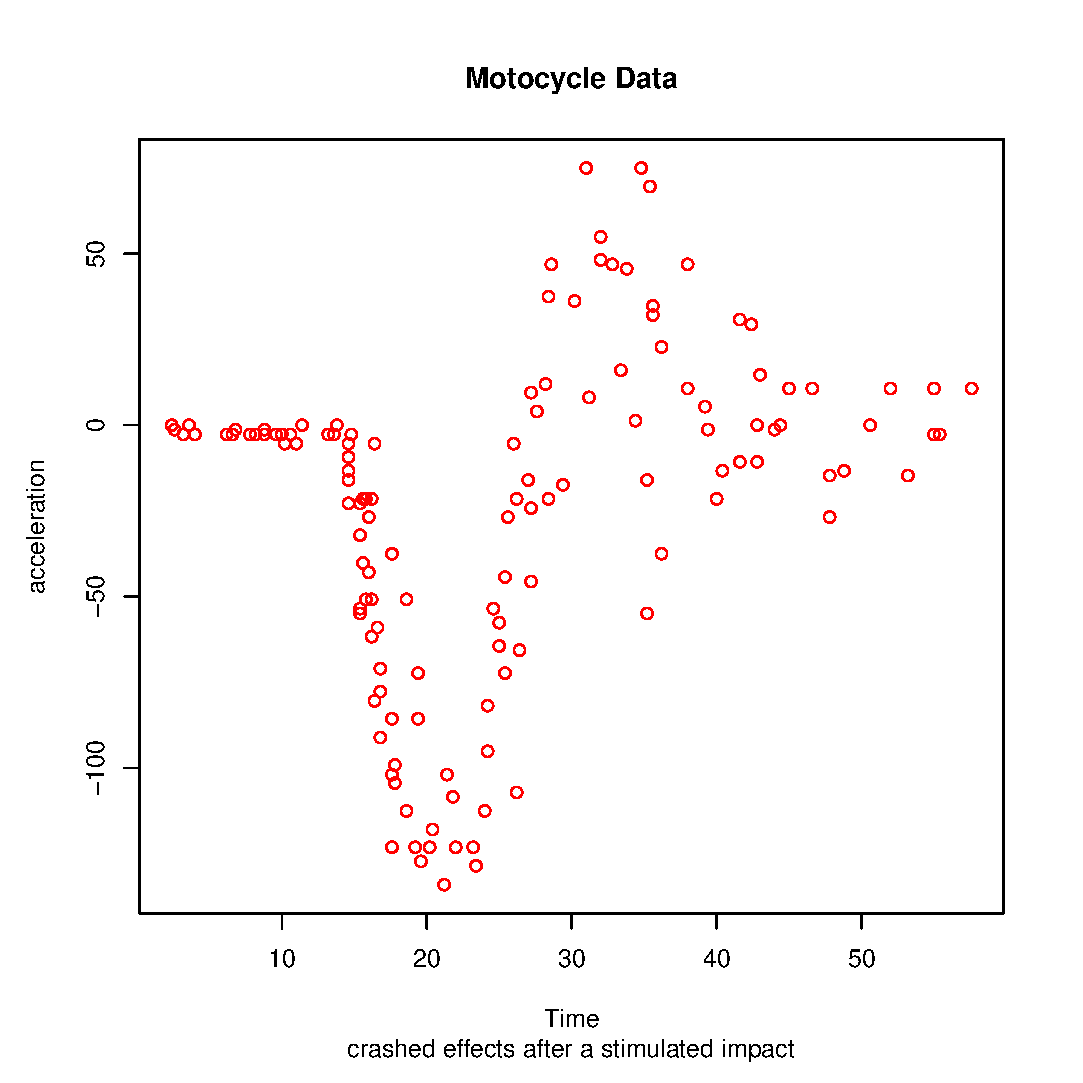
\includegraphics[width=0.75\textwidth,height=0.52\textwidth]{MotocycleData.eps}
%     \label{figure2} 

% % \end{minipage}
% \end{figure}

% \newpage
% {\LARGE{\textbf{Parametric Modeling}}}
% \vskip25pt
% {\Large\bf{Polynomial Fit}}

% \begin{figure}[h]
% % \begin{minipage}[t]{1\linewidth}
% \centering
%     %the four numbers after "trim=" are for left bottom right top
%       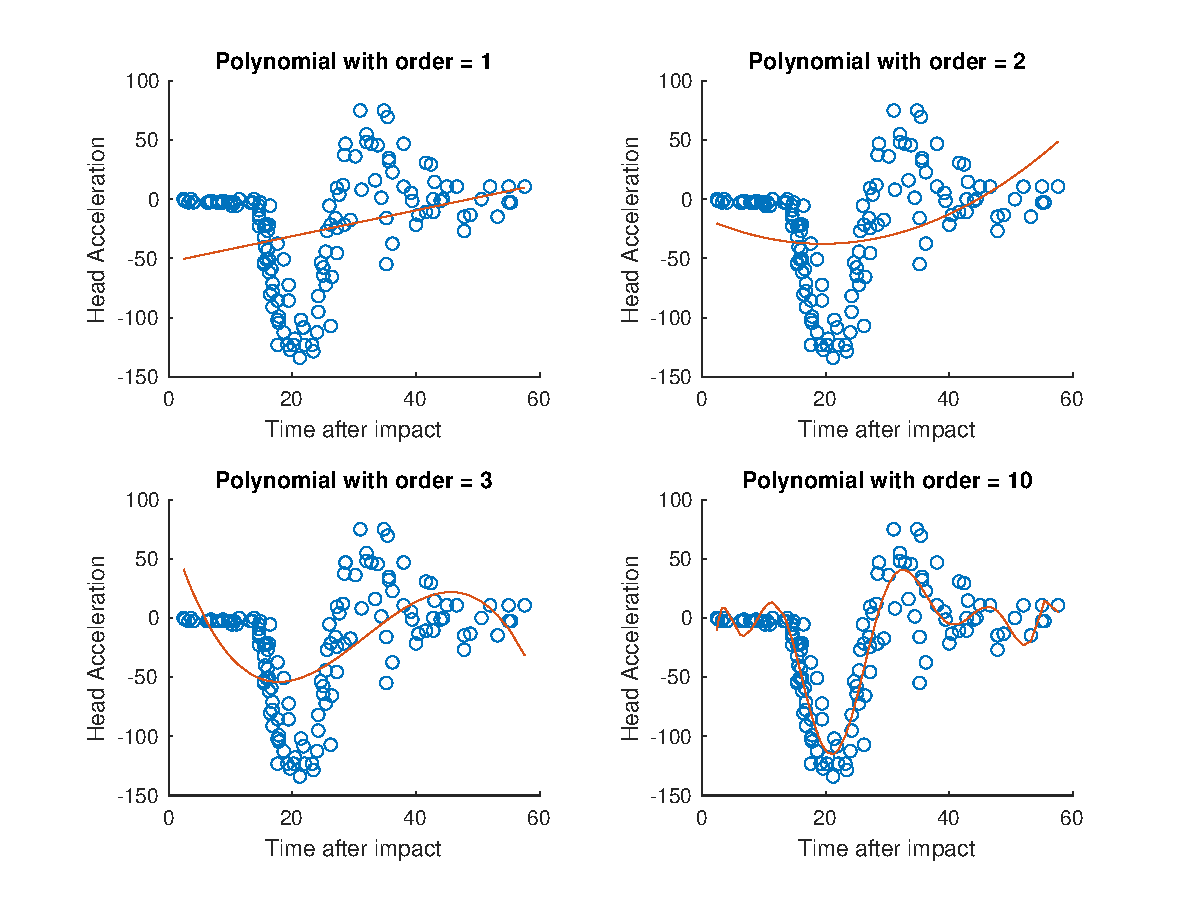
\includegraphics[width=0.75\textwidth,height=0.52\textwidth]{polyfitting.eps}
%     \label{figure3} 

% % \end{minipage}
% \end{figure}



\newpage
{\LARGE\centerline{\textbf{Pros and Cons of nonparametric method}}}
\vskip25pt
\begin{minipage}{.9\textwidth}
    \Large
\begin{itemize}
\item That makes the results more widely applicable and models more robust, i.e. nonparametric regression estimators are very flexible. There are situations when a workable parametric model is difficult to establish, for example, in biased sampling.
\item From the viewpoint of nonparametric approach, all the parametric models are too rigid. 

\item Are typically more computationally intensive, but, with our fast increasing computing power, have been made feasible and an attractive alternative to parametric methods.
\item But their statistical precision decreases greatly if several explanatory variables are included in the model, a.k.a. {\it the curse of dimensionality}.
\end{itemize}

\end{minipage}

\newpage
{\LARGE\centerline{\textbf{Summary}}}
\vskip25pt
\begin{minipage}{.9\textwidth}
    \Large
\begin{itemize}
\item Parametric models are fully determined up to one or more parameters. The statistical accuracy is guaranteed by the correctness of the underlying assumptions. 
\item Nonparametric models avoid using restrictive assumptions of the functional form of the regression function. However, they become difficult to interpret and yield inaccurate estimates if the number of regressors is large. 
\end{itemize}

\end{minipage}

\newpage
{\LARGE\centerline{\textbf{Nonparametric Methods}}}
\vskip25pt
\begin{minipage}{.9\textwidth}
    \Large Can be classified as 
\begin{enumerate}
\item classical nonparametric methods, which are based on signs and ranks developed in 1940s--1970s;
\item modern nonparametric methods, includes:
\begin{itemize}
    \item Smoothing methods, such as kernel, spline, orthogonal series for curve estimation, including density, regression curves. (Note: A curve can be regared as a parameter of infinite dimensions.)
    \item The Jackknife, Bootstrap and other resampling methods. 
\end{itemize}
\end{enumerate}
The course is mostly around the smoothing method and the curves we considered includes the density 
    % $$f(x)=\frac{\mathrm{d}F(x)}{\mathrm{d}x},$$
    and the conditional mean function.
\end{minipage}

\newpage
{\LARGE\centerline{\textbf{A toy example}}}
\vskip25pt
\begin{minipage}{.9\textwidth}
    \Large 
Suppose $\big\{(X_i,Y_i)\big\}_{i=1}^n$ is an i.i.d. sequence, with conditional mean function
$$m(x)=\E(Y_i|X_i=x)$$ 
and conditional variance $$\sigma^2(x)=\Var(Y_i|X_i=x).$$
Consider the regression 
\begin{equation}\label{L1-eq1}
    Y_i=m(X_i)+\varepsilon_i.
\end{equation}
Apparently, we have 
$$\E(\varepsilon_i|X_i)=0,$$ and
$$\E(\varepsilon_i^2|X_i)=\Var(Y_i|X_i)=\sigma^2(X_i).$$
Besides, $X_i$ and $\varepsilon_i$ are uncorrelated, i.e. orthogonal in $L^2$, but \textcolor{red}{not independent}.  (See the couterexample at the end of this slide.) 
\end{minipage}

\newpage
{\LARGE{\textbf{Example: (continue)}}}
\vskip25pt
\begin{minipage}{.9\textwidth}
    \Large 
The model in \eqref{L1-eq1} is a nonparametric regression model with the following features:
\begin{itemize}
    \item Unspecified function form for the conditional mean function $m$;
    \item Unspecified form for the distribution of $(X_i,Y_i)$ and $\varepsilon_i$;
    \item Varying variance component $\sigma^2(X_i)$.
\end{itemize}
All of those features generalizes the parametric (linear and nonlinear) regression model to more general and practical setting. 
\end{minipage}

\newpage
{\LARGE{\textbf{Nonparatric model}}}
\vskip15pt
\begin{minipage}{.9\textwidth}
    \Large 
Let $g(x,y)$ be the joint p.d.f. of $(X,Y)$. (suppose it exists of course!) The marginal p.d.f. of $X$ is 
$$f_X(x):=\int_{\R}g(x,y)\mathrm{d}y,$$
and the conditional p.d.f. of $Y$ is 
$$f_{Y|X}(y|x):=\frac{g(x,y)}{f_X(x)}.$$
The conditional mean function is closely related with the marginal density of $X$, as 
\begin{eqnarray*}
    m(x):=\E(Y|X=x)=\int_{\R}yf_{Y|X}(y|x)\mathrm{d}y=\frac1{f_X(x)}\int_{\R}yg(x,y)\mathrm{d}y.
\end{eqnarray*}

This course will start with nonparametric density estimation, and then the nonparametric estimation of the conditional mean function. 
\end{minipage}


% \newpage
% {\LARGE{\textbf{Nonparametric Modeling}}}
% \vskip25pt
% {\Large\bf{Regression Spline Fit}}

% \begin{figure}[h]
% % \begin{minipage}[t]{1\linewidth}
% \centering
%     %the four numbers after "trim=" are for left bottom right top
%       \includegraphics[width=0.75\textwidth,height=0.52\textwidth]{splinefit.pdf}
%     \label{figure4} 

% % \end{minipage}
% \end{figure}
\newpage
{\LARGE\centerline{\textbf{Counterexample}}}
\vskip25pt
\begin{minipage}{.9\textwidth}
    \Large 
    Let $p,p_1,p_2\in(0,1)$ be some constants, and $p_1\ne p_2$. Consider $X,Y$ with following distributions: 
$X\sim Bernoulli(p)$, i.e. 
$$\IP(X=1)=1-\IP(X=0)=p,$$
and $Y\sim Bernoulli(p_1)$ given $X=1$, while $Y\sim Bernoulli(p_2)$ given $X=0$. Therefore, 
$$\E(Y|X)=p_1\cdot X+p_2\cdot(1-X),$$
$$\varepsilon:=Y-\E(Y|X)=Y-[p_1\cdot X+p_2\cdot(1-X)].$$
The conditional distribution of $\varepsilon$ is
$$\IP(\varepsilon=1-p_1|X=1)=1-\IP(\varepsilon=-p_1|X=1)=p_1,$$
and  
$$\IP(\varepsilon=1-p_2|X=0)=1-\IP(\varepsilon=-p_2|X=0)=p_2.$$
\textcolor{red}{$X$ and $\varepsilon$ are not independent, but uncorrelated.}
\end{minipage}

\newpage
{\LARGE\centerline{\textbf{Counterexample(continue)}}}
\vskip25pt
\begin{minipage}{.9\textwidth}
    \Large 
    By the law of total probability, 
    \begin{equation*}
        \varepsilon=\begin{cases}
            1-p_1,~~~&\mathrm{w.p.}~~p_1p,\\
            -p_1,~~~&\mathrm{w.p.}~~(1-p_1)p,\\
            1-p_2,~~~&\mathrm{w.p.}~~p_2(1-p),\\
            -p_2,~~~&\mathrm{w.p.}~~(1-p_2)(1-p),
        \end{cases}
    \end{equation*}
 and  $\E(\varepsilon)=0$. Hence, we have 
   \begin{eqnarray*}
    \cov(X,\varepsilon)&=&\E(X\varepsilon)\\
    &=&p\E(\varepsilon|X=1)\\
    &=&p[(1-p_1)p_1+(-p_1)(1-p_1)]\\
    &=&0.
   \end{eqnarray*}
\end{minipage}

\newpage
{\LARGE\centerline{\textbf{A recap for probability theory}}}
\vskip25pt
\begin{minipage}{.9\textwidth}
   \large
\begin{defi}
    Random variables $X_1,\dots,X_n$ are called {\bf independent} if ~$\forall B_1,\dots,B_n\in\mathcal{B}(\R),$
    $$\IP(X_1\in B_1,\dots,X_n\in B_n)=\prod_{i=1}^n\IP(X_i\in B_i).$$
\end{defi}
   The correlation between $X$ and $Y$ with $\Var(X),$ $\Var(Y)>0$ is 
   $$\corr(X,Y)=\frac{\cov(X,Y)}{\sqrt{\var(X)\var(Y)}}.$$
   When the correlation is zero, one says the RVs are uncorrelated, which is NOT the same as {\bf independent}. Note 
   $$\Var(X+Y)=\Var(X)+\Var(Y)~~\Leftrightarrow~~\cov(X,Y)=0.$$
 Again, independence implies uncorrelated, but not the other way around: uncorrelated RVs don't need to be independent! (See the counterexample!)
   
   \vskip 5pt
   But for Gaussian $(X,Y)$, it's the same, i.e. {\it independent} is equivalent to {\it uncorrelated}. 
\end{minipage}

\newpage

\newpage
{\LARGE\centerline{\textbf{Appendix: Some Concepts}}}
\vskip25pt
% \begin{minipage}{.9\textwidth}
   \large

% \end{minipage}


For a sequence $\left\{M_n\right\}$ of random variables, the following concepts are usually considered in statistical theory.

\begin{itemize}


\item \underline{\bf converge in mean square}

\begin{itemize}

\item Definition: if there is a random variable $ \xi $,such that
$$
\lim_{n\to \infty } \mathbb{E} (|M_n - \xi|^2)=0
$$
then we say that $ M_n $ converges to $ \xi $ in mean square. Denoted by
$$
M_n \stackrel{L^2}{\rightarrow} \xi
$$

\item \underline{\bf mean square consistent estimator}:  suppose $ \theta $ is a parameter (or a function), if $ M_n $ converges to $ \theta $ in mean square, then we say that $ M_n $ is a mean square consistent  estimator of $  \theta $


\item  \underline{\bf (mean square) consistent rate}: If $M_n$ is a consistent estimator of $ \theta $,  and there exists an $ a_n \to 0 $ such that 
$$
  \mathbb{E} (|M_n - \xi|^2) = O(a_n^2),
$$
Then, we say that $a_n $ is the consistence rate of $ M_n$.

\item Example 1: Suppose $ X_1, ..., X_n $ are i.i.d. samples from $ X $ with $ \E(X) = \mu $ and $ \Var(X) = \sigma^2 $. Then 
    $$
      \E [(\bar X - \mu)^2]  = \sigma^2/n  
    $$
    Thus, $ \bar X$ is a consistent estimator of $ \mu $ in mean square, and the consistency rate is $ 1/\sqrt{n} $, also called root-$n$ consistent.
\item Example 2: The empirical distribution $\hat{F}_n(x)$ is an consistent estimator of $ F(x) $ in mean square and the consistency rate is $1/\sqrt{n}$, a.k.a. root-$n$ consistent.

Proof: because
$$
    \mathbb{E}(\hat{F}_n(x)) = F(x)
$$
and 
\begin{align*}
  \mathbb{E}\left[ \left|\hat{F}_n(x) - F(x)\right|^2 \right] &= \Var(\hat{F}_n(x))\\
  & = \frac{F(x)(1-F(x))}n \\
  & \to 0,
\end{align*}
thus $\hat F_n(x)$ is a consistent estimator of $ F(x) $ in mean square.

\newpage


\item \underline{\textbf{MSE (mean squared error)}} If $ M_n $ is an estimator of $ \theta $, we also call $\E [(M_n - \theta)^2] $ the mean squared error,
    \begin{align*}
      {\rm MSE}(M_n) = \E [(M_n - \theta)^2] 
    \end{align*}

\item Therefore, if $ M_n $ is an estimator of $ \theta $ with MSE tends to 0, then $ M_n $ is an consistent estiamtor of $ \theta $ in mean square.
    

\item \underline{Decomposition of MSE} 
    \begin{align*}
      {\rm MSE}(M_n) &= \E [(M_n - \theta)^2] \\
               & = \E [(M_n - \E M_n +E M_n- \theta)^2] \\
               & = \E [(M_n - \E M_n)^2 + (\E M_n- \theta)^2 + 2 (M_n - \E M_n)(  \E M_n- \theta)]  \\
               & = \E [(M_n - \E M_n)^2] + (\E M_n- \theta)^2   \\
               &= \Var(M_n) + {\rm Bias}(M_n)^2
    \end{align*}
   

\end{itemize}

%\item By the fact above, $\hat F_n(x)$ is a consistent estimator of $ F(x) $ in probability.




\newpage


\item \underline{\bf convergence in probability}. 

\begin{itemize}

\item Definition: If  $ \xi $ is a random variable, and for all $\varepsilon>0$
$$
\lim _{n \rightarrow \infty} \mathbb{P}\left(\left|M_n-\xi \right|>\varepsilon\right)=0,
$$
then we say that $M_n$ converges to $ \xi $ in probability. Denoted by
$$
M_n \stackrel{p}{\rightarrow} \xi, \ \ \ 
or
\ \ \ 
M_n {\rightarrow} \xi \ \ \  (i.p.).
$$

\item {\bf A basic fact}, if $M_n $ converges to $ \xi $ in mean squares, then $M_n $ also converges to $ \xi $ in probability. In fact, convergence in $L^p$ sense always implies convergence in probability, for any $p>0$. See \cite[Theorem~4.1.4]{chung00} for more details. 
    
    \begin{itemize}
    
    \item   Markov's (Chebyshev's) inequality: for any random variable $ X$, if the second moment exists, then
    $$
     \IP(|X|>\varepsilon) \le \frac{\E(X^2)}{\varepsilon^2}
    $$
    
    \item replace $ X $ by $M_n - \xi $
    $$
     \IP(|M_n - \xi |>\varepsilon) \le \frac{\E(|M_n - \xi |^2)}{\varepsilon^2}
    $$
     
    \item Thus $\E(|M_n - \xi |^2) \to 0$ implies the left hand side tends to 0
    
    \end{itemize} 

\newpage

\item \underline{\bf consistent estimator in probability}:  suppose $ \theta $ is a parameter (or a function), if $ M_n $ converges to $ \theta $ in probability, then we say that $ M_n $ is a consistent estimator of $
\theta $ in probability. 

\item Example: by the fact above, $ \bar X $  and $ \hat F_n(x) $  are consistent estimator of $ \mu $ and $ F(x) $ in probability, respectively.

\end{itemize}
\item  \underline{\bf convergence with probability 1} (w.p.1). If there exists an event $A\subseteq\Omega$ with $\IP(A)=1$ such that $\forall~\omega\in A$, we say that $ M_n $ converges to $ \xi $ with probability 1 (or almost surely)
$$
M_n \stackrel{a.s.}{\rightarrow} X.
$$
or 
$$
M_n {\rightarrow} X, \ \  a.s. .
$$

\item[] {\bf strong consistency of an estimator}:  suppose $ \theta $ is a parameter (or a function), if $ M_n $ converges to $ \theta $ a.s., then $ M_n $ is a strong consistent (or almost surely) estimator of $  \theta $.

\item {\bf  converges in distribution}:
\begin{itemize}
  \item  Definition: 
 if 
$$
\lim_{n\to \infty } \IP(M_n\le x) = \IP(\xi\le x)
$$
at all points $x\in\R$ where the c.d.f. $F_\xi(x):=\IP(\xi\le x)$ is continuous, 
then we say that $ M_n $ converges to $ \xi$ in distribution, denoted by
$$
M_n \stackrel{d}{\rightarrow} \xi. 
$$

\item A special case is $ \xi \sim \mathcal{N}(\mu, \sigma^2)$, in that case we also write
$$
M_n \stackrel{d}{\rightarrow} \mathcal{N}(\mu, \sigma^2).
$$


\item \underline{\bf central limit theorem} Let $X_1, X_2, X_3, \ldots$ be a sequence of independent and identically distributed (i.i.d.) random variables with a finite mean $\mu$ and finite variance $\sigma^2$, then
$$
   \frac{\bar X- \mu}{\sigma/\sqrt{n}}  \stackrel{d}{\rightarrow} \mathcal{N}(0, 1)
$$
%where $ \xi $ is any random variable following $\Phi(\mathrm{x})$ is the cumulative distribution function of the standard normal distribution.

\item Example 1: estimator of the CDF $ \hat F_n(x) $:
$$
  \hat F_n(x) - F(x)  \stackrel{d}{\rightarrow} \mathcal{N}\left(0, \frac{F(x)(1-F(x))}n\right)
$$
or
$$
 \sqrt{n} \frac{\hat F_n(x) - F(x)}{\sqrt{F(x)(1-F(x))}}  \stackrel{d}{\rightarrow} \mathcal{N}(0, 1).
$$



\end{itemize}


\end{itemize}

\newpage


\bibliographystyle{apalike}
\bibliography{ref}
% \begin{thebibliography}{}

%     \bibitem[Hall, 2013]{Hall13}
%     Hall, P. (2013).
%     \newblock {\em The bootstrap and Edgeworth expansion}.
%     \newblock Springer Series in Statistics. Springer New York, NY.
    
%     \bibitem[H{\"a}rdle et~al., 2004]{hardle04}
%     H{\"a}rdle, W., M{\"u}ller, M., Sperlich, S., Werwatz, A., et~al. (2004).
%     \newblock {\em Nonparametric and semiparametric models}, volume~1 of {\em Springer Series in Statistics}.
%     \newblock Springer Berlin, Heidelberg.
    
%     \bibitem[Kloke et~al., 2015]{kloke14}
%     Kloke, J., McKean, J.~W., and McKean, J.~W. (2015).
%     \newblock {\em Nonparametric statistical methods using R}.
%     \newblock Chapman and Hall/CRC, 1st ed edition.
    
%     \bibitem[Schmidt et~al., 1981]{schmidt81}
%     Schmidt, G., Mattern, R., and Sch{\"u}ler, F. (1981).
%     \newblock Biomechanical investigation to determine physical and traumatological differentiation criteria for the maximum load capacity of head and vertebral column with and without protective helmet under the effects of impact.
%     \newblock {\em EEC Research Program on Biomechanics of Impacts, Final report, Phase III, Project G}, 5.
    
%     \bibitem[Scott, 2015]{scott15}
%     Scott, D.~W. (2015).
%     \newblock {\em Multivariate density estimation: theory, practice, and visualization}.
%     \newblock Wiley Series in Probability and Statistics. John Wiley \& Sons, 2nd edition.
    
%     \bibitem[Silverman, 1985]{Silverman85a}
%     Silverman, B.~W. (1985).
%     \newblock Some aspects of the spline smoothing approach to non-parametric regression curve fitting.
%     \newblock {\em Journal of the Royal Statistical Society: Series B (Methodological)}, 47(1):1--21.
    
%     \bibitem[Takezawa, 2005]{takezawa05}
%     Takezawa, K. (2005).
%     \newblock {\em Introduction to nonparametric regression}.
%     \newblock Wiley Series in Probability and Statistics. John Wiley \& Sons.
    
%     \end{thebibliography}
    
\end{document}